\documentclass[12pt]{report}
\linespread{1.5}
\usepackage{graphicx}
\usepackage{fullpage}
\usepackage{natbib}
\usepackage{float}

\bibpunct{[}{]}{,}{a}{,}{,}

\begin{document}

\title{Developing a Compiler for the Expert Systems Language, Flex}
\author{05017742 - Thomas Cowell\\
		\texttt{05017742@glam.ac.uk}}

\maketitle

\begin{abstract}
The aim of this project is to create a simple compiler for the expert systems language, Flex.  Flex is an expert systems language that focuses on using plain English to make it accessible for non-technical users, and to aid building rapid rule based systems.
\end{abstract}

\pagestyle{plain}
\pagenumbering{alph}

\tableofcontents

\cleardoublepage
\pagenumbering{arabic}

\chapter{Introduction}

\section[Why This Project?]{Why This Project?}\label{sec:why_this_project}
Before this paper begins, it is worth noting the motivation behind this project.  Certain modules on the 'Intelligent Computer Systems' course required the use of a propietary software package called WinProlog.  The application can do a wealth of tasks, however, the modules only focused on a niche feature of the software, a toolkit based on Prolog called Flex (not to be confused with the lexical analysis tool, or Adobe's Software Development Kit, also of the same name).  Win-Prolog's Flex allows professionals, engineers and students alike to quickly write a rule-based system using a language that is very close to the English language.
\\*
\\*
Whilst flex achieved results, it was felt that the debugging features were sub-par and were often inaccurate, giving no helpful messages for a beginner to use to correct their mistakes.  Also, because of the restrictions of having a licence, it meant that the software could only be installed on certain machines, in a different department within the University campus, which students felt was restrictive and inconvienient.
\\
\\
\\
\\
\begin{figure}[h!]
	\centering
		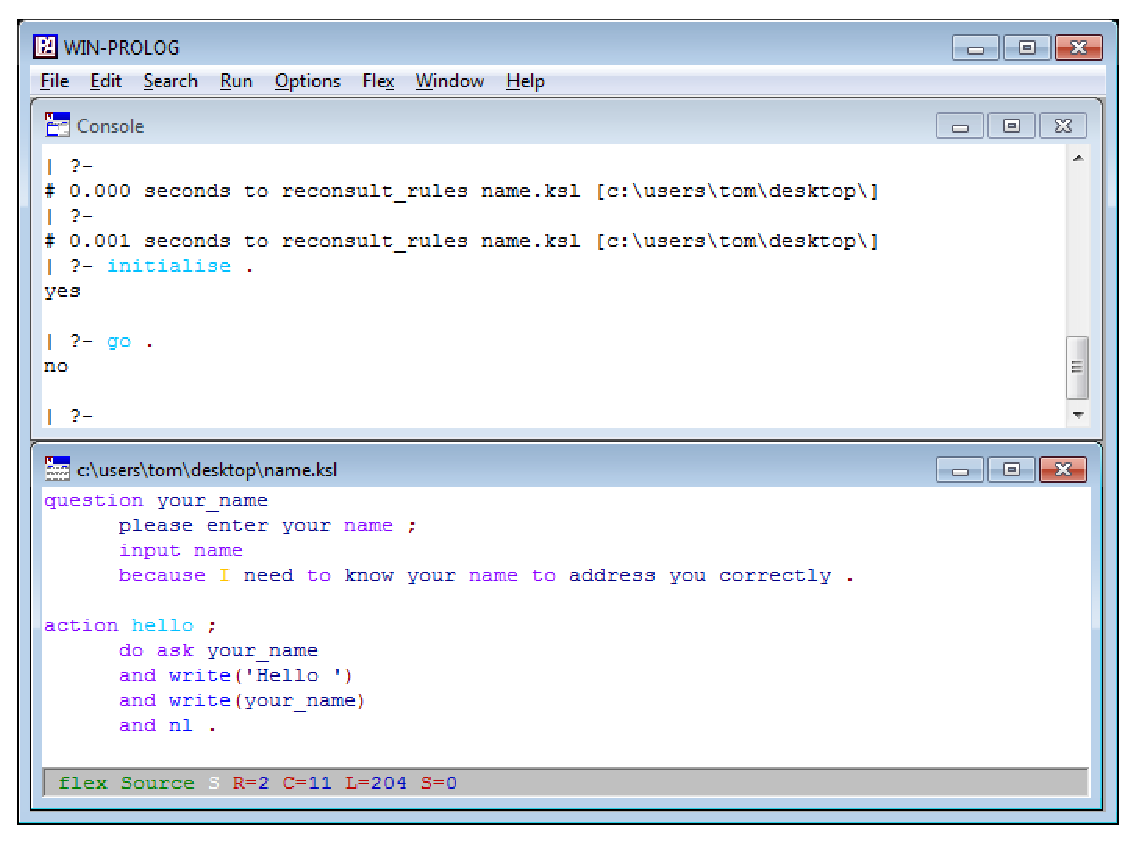
\includegraphics[scale=0.85]{flexfail}
		\caption{A simple flex program that is syntatically wrong, plus the resulting error.}
\end{figure}
\\
In figure 1.1, the line \texttt{input name} should have a semi-colon at the end, like \texttt{input name ;}, to let the compiler know that the line is finsihed, but the question isn't over.  Whilst this is a simple mistake, the flex compiler hasn't picked it up, and is only being discovered when trying to run the action \texttt{go}, where flex returns an error message \texttt{no}, with no indiciation what the error is, where it is or how to fix it.  If this were a large set of rules, finding such a basic mistake could take a long time to fix.
\\*
\\*
The examples below show flex encountering a gramatically incorrect script, with the compiler displaying errors.
\begin{figure}[h]
	\centering
		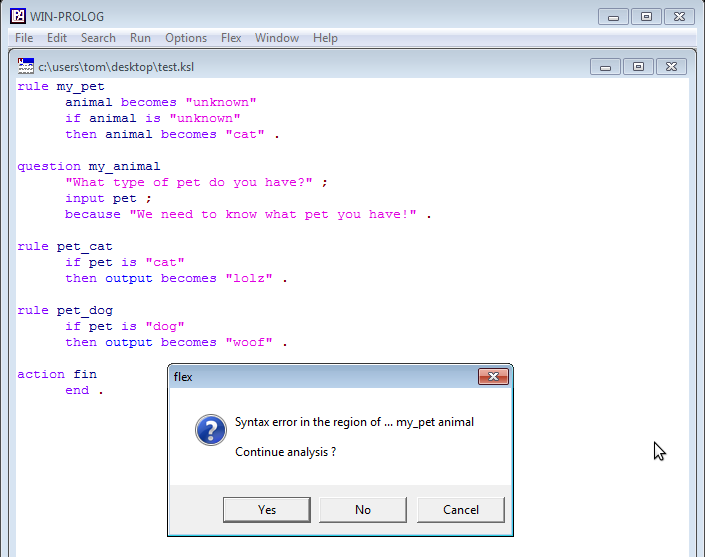
\includegraphics[scale=0.65]{flex_error1}
		\caption{The compiler has detected an error in the grammar.}
\end{figure}
%\\*
%\\*
What we see here is some random text talking about nothing much at all!
\begin{figure}[ht]
	\centering
		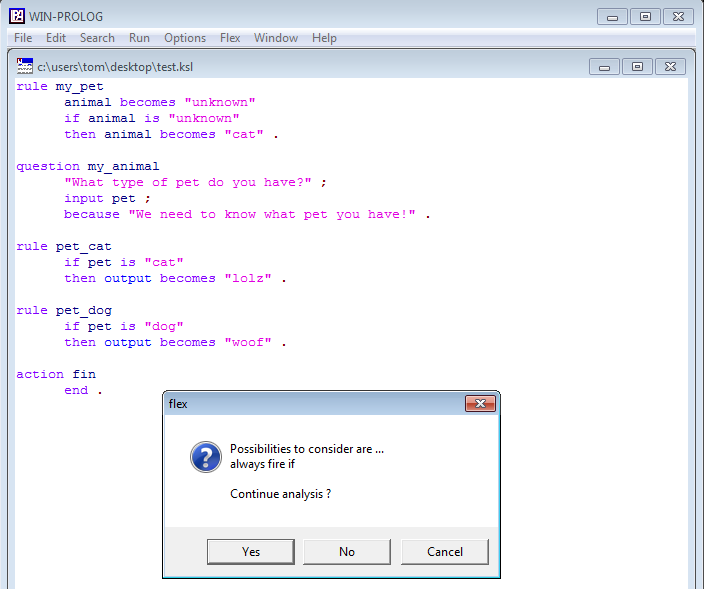
\includegraphics[scale=0.65]{flex_error2}
		\caption{The compiler error isn't very specific to where it is refering to, there are no line number or highlighting on the error.}
\end{figure}
\\*
Whilst the compiler in WinProlog does try to track down the error, it's not very friendly to new users, as it doesn't let them know where the error is, or what is wrong.  There were situations where n tutorials and in courseworks, where by small, simple errors could have been easily fixed if it weren't for ambiguous language on the debugger.
\clearpage
\section{Aim}\label{sec:aim}
The problems outlined in the previous section help highlight the aims and objectives that this project can use.  Time is limited, so it wouldn't be wise to implement a full version of Flex, however a small subset of the language would be sufficient.
\\
\\
This project aims to create a basic implementation of the flex toolkit, using open source software.  The software would be able to be installed on any linux machine, whilst providing the basic features required to teach students how to write expert systems.
\section{Objectives}\label{sec:objectives}
The objectives of this project are to:
\begin{itemize}
\item Create a simple flex interpreter that can work on the simple tutorials from a tutorial.
	\begin{itemize}
	\item Recognise rules, questions and actions;
	\item Recognise variables, assignments and comparisons;
	\item Work with simple if-statements
	\item Output variables and text using the write() statement.
	\end{itemize}
\item Create it for the Linux platform.
	\begin{itemize}
	\item Command line driven - feed the application a flex source file.
	\item Not be coupled to a Desktop Environment (Gnome, KDE etc).
	\end{itemize}
\item Keep the project open source.
	\begin{itemize}
	\item Keep the project available on a source-control service so it can be ammended to once the project is finished.
	\end{itemize}
\end{itemize}

\section{Project Overview}\label{sec:project_overview}
This project shall begin by looking into the previous or similar research that others have carried out on this topic.  Reseach will then be conduced into Expert Systems, Win-Prolog and flex, with sample scripts of what it is capable of.  Adding to this, research will then be conducted into the tools used to write a compiler.  The implementation of the compiler will also be documented.

\chapter{Literature Review}
\section{Outline}\label{sec:outline}
As described in the previous chapter, the outline of this project is to create a compiler for the expert systems language, flex.  Whilst Flex is based on the Artificial Intelligence langauge Prolog, this basic compiler will be written in C, emulating the basic features of flex, mainly as a teaching tool, rather than a fully fledged toolkit.  However, because Flex is built on top of Prolog, there are many papers on writing Prolog compilers.

\section{Previous Work}\label{sec:previous_work}
Because the Flex toolkit is unique, there aren't many examples or previous work done on creating a compiler soley for Flex.  However, there are countless items of literature dedicated to writing compilers, all for different languages, but constructed in the same manor - using Flex and Bison.

\chapter{Research}
\section[Research]{Research}\label{sec:intro_to_research}
Before any implementation can begin, research needs to be conducted in order to gain better knowledge about expert systems, the Flex language and various toolkits for developing interpreters.

\section{Expert Systems}\label{sec:expert_systems}
In the modern world where information is highly valuable and where time is of the esence, many experts have turned to computing to help provide answers for them that may otherwise take a while to reach through their own expertese.  Expert Systems provide an easier way for professionals to reach conclusions through a series of questions, usually linking to a knowledge base.  For example, a doctor may use an expert system to reach a diagnosis for a patient, where the illness or problem may not be readily obvious.  The system would ask a question, where the doctor would answer with the symptoms, and then the expert system would continue asking more questions, based on the previous answers, until a conclusion is reached.
\\*
\\*
Expert system development entials the conversion of information about a bounded problem domain into knowledge, which is then represented in a format suitable for computer manipulation.  The created depository of knowledge, known as the knowledge base, can then by used by various deductive reasoning techniques to derive solutions \citep{expertsystems98}.
\\*
\\*
From this, it is obvious that the usefulness of the expert system is only as good as the underlying data - the knowledge base.  Using the doctors example from the previous paragraph, the system would be of no use if the knowledge base was minimal, whilst in the reverse situation, it would be extremely useful to have a large knowledge base.  Doctors from around the world could contribute answers as new illnesses and cures are discovered, which in turn would improve the accuracy and usefulness of the expert system.
\\*
\\*
Expert systems can be found in many areas of industry, including engineering, medical, financial forecasting, or even just personal information systems for helping customers at a shopping centre.
\\*
\\*
Expert systems languages are entirely different to imperative languages such as C, C\#, Java.  Instead, they make use of logical langauges, such as Prolog, which is based on rules, and assosciations with data.  The code in figure \ref{fig:prolog_code} shows a short example of a program written in Prolog.
\\*
\\*
\begin{figure}[H]
\texttt{born(charles, elizabeth2, philip).\\
born(anne,    elizabeth2, philip).\\
born(andrew,  elizabeth2, philip).\\
born(edward,  elizabeth2, philip).\\
\\
born(diana,   frances,    edwardSpencer).\\
\\
born(william, diana,      charles).\\
born(henry,   diana,      charles).\\
\\
? born(S, elizabeth2, Y) and born(G, M, S).}
\caption{Example Prolog code.\citep{thehouseofwindsor}}
\label{fig:prolog_code}
\end{figure}
The first four lines link the first argument with the next two.  So, on line one, charles is the child of elizabeth2 and philip.  On the 5th line, diana is declared as the daughter of frances and edwardSpencer 
The final line execute the program, by submitting a query.
\\*
\\*
\begin{figure}[H]
\texttt{born(charles, elizabeth2, philip), born(william, diana, charles) yes\\
born(charles, elizabeth2, philip), born(henry, diana, charles) yes}
\caption{Output from executing the sample code.}
\label{fig:prolog_output}
\end{figure}
Figure \ref{fig:prolog_output} shows the output from the sample code.  The query executes two sub queries, \texttt{born(S, elizabeth2, Y)}, which retrives a set of data where the child's mother is \texttt{elizabeth2}.  Based on the four rules at the start of the program, this would return four answers for \texttt{S}, and a single result for \texttt{Y} (philip).  The second query, \texttt{born(G, M, S)} queries the returned data set from the first query.  In this case, the mother (\texttt{M}), while the father is \texttt{S}.  Lines six and severn in \ref{fig:prolog_code} show that charles has two children, and thus \texttt{william} and \texttt{henry} are returned.
\clearpage
\textbf{Disadvantages}\\
There are some notable disadvantages to expert systems.  An important pitfall to consider is the GIGO acronym - Garbage In Garbage Out.  If the rules are .  Also, if the person being questioned gives an answer that they're uncertain of, then the result may not be accurate, and the expert system would be non-the wiser.  A human expert would be able to tell the certainty of someones answer, and possibly re-ask the question in a way that the questionee would understand.

\subsection{WinProlog}\label{subsec:winprolog}
WinProlog is a propietary software package, developed by Logic Programming Associates Ltd.  LPA describe Win-Prolog below:
\\*
\\*
WIN-PROLOG is the leading Prolog compiler system for Windows-based PCs. Prolog is an established and powerful AI language which provides a high-level and productive environment based on logical inference.\citep{lpawinprolog}
\\*
\\*
One of the features of Win-Prolog is Flex, an expert systems toolkit built on top of Prolog.

\subsection{Flex}\label{subsec:flex}
The 'Flex Tutorial' describes Flex as "Flex is a software system specifically designed to aid the development and delivery of Expert Systems."
\\*
\\*
To appreciate both the power and limitations of Expert System approaches to reaching expert conclusions, it is necessary to construct and experiment with expert systems.  In this module, the Flex Expert System Shell will be used.  Flex describes knowledge in terms of \textit{production rules} (that is, \textit{if-then} statements), which has proved the most popular approach to encapsulation expert knowledge.  Such rules, despite appearing simple, enable relatively complex connections to be made between individual pieces of 'knowledge', thereby solving apparently difficult problems.\citep{flexsystems09}.
\\*
\\*
The advantages of flex is that it's easy to understand, as it's very close to the English language.  A non-programmer could look at it and understand the system within several minutes, where as a traditional Prolog script may need some understanding of programming to be able to understand what is going on.
\\*
\\*
Flex expert system toolkit, an expressive and flexible rule-based development system for building and delivering scalable and flexible expert systems and business rules applications. Flex provides a comprehensive and versatile set of facilities for both programmers and non-programmers to construct reliable and maintainable applications.\citep{lpawinprolog-flex}.
\\*
\\*
The code below shows an example program written in flex:
\begin{figure}[H]
\texttt{\begin{tabbing}group \= temperature\_choices warm, cold .\\
\\
rule ask\_temperature \\
\>	if the temperature is unknown\\
\>	then ask temperature .\\
\\
question temperature\\
\>	What is the temperature?;\\
\>	choose from the temperature\_choices ;\\
\> 	because it is necessary to work out the need for a coat .\\
\\
rule temp\_w\\
\>	if temperature is warm\\
\>	then write('You would be mad to wear a coat.').\\
\\
rule temp\_c\\
\>	if temperature is cold\\
\>	then write('Take a coat to keep warm.').\\
\\
ruleset take\_a\_coat\\
\>	contains all rules;\\
\>	select rule suing first come first servced;\\
\>	update ruleset by removing each selected rule;\\
\>	initiate by doing restart .\\
\\
action go\\
\>	do invoke ruleset take\_a\_coat .\\
\end{tabbing}}
\caption{A simple flex program that lets you know if you should wear a coat or not.\citep{flexsystems09}}
\label{fig:flex_code}
\end{figure}
It's immediately obvious that the program is made up of rules and questions.  The compiler starts from the top, and runs down through the rules, until they've all been fired.  Questions only get fired if they are called upon within a rule.\\*
\\
The first line declares a group of choices that can be asked during a question.  This can be likened to a Enumerative type in languages such as C and C\#, where \texttt{warm} and \texttt{cold} are two options that belong to \texttt{temperature}.  The first rule, \texttt{ask\_temperature}, checks if the variable \texttt{temperature} (not to be confused with the group of the same name) has been assigned a value.  If it's not, then it asks the question, \texttt{temperature}.  Because the flex compiler starts at the top, then temperature will be unknown by default, so this rule will always fire.\\
\\
Questions always have the same format: The first line is the question text that the user will see, the second line presents the options to the user and also accepts their input.  In this instance, the user will be presented the two choices of \texttt{temperature}, where the choice is then assigned to the variable \texttt{temperature}.\\
\\
The two rules, \texttt{temp\_w} and \texttt{temp\_c}, check the users input, and display the message as appropriate, while the ruleset \texttt{take\_a\_coat} tells the compiler how to go about running the script.  Finally, the the action \texttt{go}, which is triggered as a query from the command prompt, starts the program.\\
\\
Whilst this is a reasonably simple script, it has all the basics that make up larger and more complicated flex programs.

\section{What Is A Compiler?}\label{sec:what_is_a_compiler}
Programming languages are notations for describing computations to people and to machines.  The world as we know it depends on programming langauges, because all the software running on all the computers was written in some programming langauge.  But, before a program can be run, it first must be translated into a form in which it can be executed by a computer.

The software systems that do this translation are called \textit{compilers}.\citep{compilers07}
\\*
\\*
This quote nicely gives a brief overview of what a compiler does.  It translates the human readable program into a format that the computer can understand, i.e. instructions.  Whilst this sounds simple, the actual process is reasonably complicated, and done in several phases:\\
\begin{itemize}
	\item Lexical Analysis
	\item Syntactical Analysis
	\item Intermediate Code Generation
	\item Optimization
	\item Object Code Generation
\end{itemize}\citep{compilerconstruction92}
\subsection{Lexical Analysis}\label{subsec:lexical_analysis}
The first task of the compiler is to read the source code that the developer has written, and breaks it up into meaningful chunks called tokens.  These tokens are defined in a lexical file, in which the lexical scanner will process.
\\*
For example, take the following flex code:\\*
\texttt{\begin{tabbing}rule \= my\_pet\\
\>	if animal is 'cat'\\
\>	then sound becomes 'meow' .\\
\end{tabbing}}
This can be broken down to be easier to understand:\\*
\begin{itemize}
	\item keywords: rule, if, is, then
	\item identifiers: my\_pet, animal, sound
	\item operator: becomes
	\item string: 'cat', 'meow'
	\item punctuation: .
\end{itemize}
The lexical analyiser is capable of removing characters that aren't relevant to the program, such as comments, new lines and whitespace (spaces and tabs).  All of the above are leximes that are mapped into tokens, that makes it easier for the syntactical analyser to understand.  The way that the lexical analyser recognises these leximes is through matching the patterns of text, which is where regular expressions come in useful.\\
\subsubsection{Regular Expressions}\label{subsubsec:regex}
Regular Expressions, or more commonly known as 'regex', allows developers to match patterns of text.  It is extremely powerful for recognising patterns in text, and thus, is used in the lexical analysus process for matching expressions to create tokens.
\\*
\\*
A regular expression is a pattern description using a metalanguage, a language that you can use to describe what you want the pattern to match.  Flex's regular expression language is essentially POSIX-extended regular expressions (which is not surprising considering their shared Unix heritage).\citep{flexandbison09}
\\*
\\*
Regular expressions are a powerful way of matching complicated patterns of strings.  It uses a series of special characters that allow the user [of regular expressions] to create a query.
\\*
For example, numbers can be expressed in several ways, some numbers are negative and some have decimal places.  An expression needs to be able to recognise these different formats.  A string of digits, which can either be positive or negative, can be represented using the expression below:\\*
\\*
\texttt{[-+]?[0-9]+}
\\*
\\*
The square brackets \texttt{[ ]} represents a character class, matching anything within the brakcets.  The first occurance, \texttt{[-+]} matches either a postive of a negative symbol at the start of the expression.  The \texttt{?} character means that the preceding character class can either occur once, or never, which means that the plus or minus characters can be optional.  Next is the \texttt{[0-9]} expression, which matches any text that is number 0 to 9 - the \texttt{+} at the end means that the preceeding expression can be matched one or more times, allowing a number to be either 1 or 12345.  Another example, shown below, recognises an identifier, such as one from the flex example.
\\*
\\*
\texttt{[a-zA-Z\_][a-zA-Z0-9\_]*}
\\*
\\*
The expression is comprised of two character classes.  The first matches a series of characters, in either lower or uppercase, followed by an underscore. The following class is similar, but can also contain numbers.  The astricks, \texttt{*}, means that the preceeding expression can be matched zero or more times, so, the second character class is optional.  This example allows for an identifier to look something like:\\
\\
\texttt{animal}\\
\texttt{My\_Animal01}\\
\texttt{animal\_}\\
\\
But \textbf{not}:\\
\texttt{my1\_animal}\\
\texttt{1\_animal}\\
\\
Matching keywords is much easier, as they need to be treated literally.  Matching for the \texttt{if} keyword, for example, simply looks like so:\\*\\*
\texttt{"if"}
\subsection{Syntactic Analysis}\label{subsec:syntactical_analysis}
The process of syntactic analysis is to parse the tokens into meaningful sentences.  It creates a tree of tokens, whereby each node represents an operation such as \texttt{while}, and its child nodes represent the evaluation expression, and the block of code to loop around, which could be broken down again, where the evaluation is the root node, and the children are the parameters and comparison operators.
\begin{center}
\texttt{\begin{tabbing}while \= (found != true) \{\\ \> found = do\_something();\\ \}\end{tabbing}}
\end{center}
The code above can be broken down into tokens.
\begin{itemize}
	\item Keywords: while, true
	\item Identifiers: found, do\_something
	\item Operators: =
	\item Comparison: !=
	\item Punctuation: \{ \} ( ) ;
\end{itemize}
\begin{figure}[H]
	\centering
	\includegraphics[scale=1]{whilegraph}
	\caption {Expression parse tree.}\label{fig:whilegraph}
\end{figure}
Figure \ref{fig:whilegraph} shows a parse tree of the simple \texttt{while} code sample.  The code is broken down into two main parts - the evaluation, and the block.  These are then further broken down further down the tree.
\\*
The syntactic analyzer, or \textit{parser}, is the heart of the front end of the compiler.  The parser's main task is analyzing the structure of the program and its component statements and checking these for errors.  It frequently controls the lexical analyzer, which provides tokens in response to the parser's requests, and it may also supervise the operation of the intermediate code generator.\citep{compilerconstruction92}
\\*
\\*
A programming langauge follows a strict set of rules that form it, much like the English langauge has rules to string certain words together to form meaningful and sensible sentences.  The parser's job is to put the tokens into an order that follows the grammar.  For example, the grammar specifies that an identifier, or an expression, must come after the \texttt{if} keyword, followed by a comparison of another identifier or expression.
\subsubsection{Grammar}\label{subsubsec:grammar}
The grammar is the important area of the parser, as it defines how the langauge should look and work.  Most langauges use "context free grammars", whereby the grammar is built up in steps, to provide a bigger picture.
\subsection{Intermediate Code Generation}\label{subsec:intermediate_code_gen}
Bing bish bash bosh
\subsection{Optimization}\label{subsec:optimization}
Bing bish bash bosh
\subsection{Object Code Generation}\label{subsec:object_code_gen}
Bing bish bash bosh
\section{Development}\label{sec:development}
\subsection{Environment}\label{subsec:dev_environment}
One of the main aims of this project was to create an open-source alternative to the propietary package "WinProlog", which provides the Flex toolkit.  This aim was to provide the project on an open-source platform, such as Linux, which would allow lecturers to tailor the package to their needs, allowing them to fix any bugs or add more advanced features, without the fear of violating any licences.  Therefore, Linux was the platform of choice to develop on, where the distribution of choice was Ubuntu, as it has a great wealth of development applications in its repositories, such as \texttt{flex}, \texttt{bison} and \texttt{gcc}.  Ubuntu provides a package, \texttt{build-essential}, to help developers write and compile applications easily, which contains many useful tools that should please a large majority of software developers.\\*
\\*
Installing these packages in Ubuntu simply required the following command:
\\*
\\*
\texttt{\$ sudo apt-get install flex bison build-essential}
\\*
\\*
Flex and Bison shall be discussed in the next chapter.  \texttt{build-essential} is a Debian meta-package, that is, it is simply a list of packages that are essential to building applications in a Debian based distribution.  The package satifisies the needs for most developers wishing to develop applications on Linux, and includes packages such as \texttt{gcc} and \texttt{g++} - a C and C++ compiler, respectively.
\\*
\\*
Ubuntu provides a wealth of choice when it comes to development tools, however only the simple tools are required, such as a text editor such as \texttt{gedit}, or console based text editor, \texttt{nano}, whilst the terminal is perfectly acceptable for running commands to compile the tokens, grammar and C program together.  \texttt{make} comes part of the \texttt{build-essential} package, which allows a developer to write a series of commands into a makefile, and then simply run the command:\\*\\*
\texttt{\$ make}
\\*
\\*
in the directory where the makefile is located.
\subsection{Flex}\label{subsec:flex}
Bing bish bash bosh
There are several incarnations of lexical analysis programs, but the most popular is Flex, which originally dirived from yacc and lex.  Lex was written in 1975 by Mike Lesk and Eric Schmidt (now CEO of Google Corporation)

Flex and Bison are tools for building programs that handle structured input.  They were originally tools for building compilers, but they have proven to be useful in many other areas.\citep{flexandbison09}.
\subsection{Bison}\label{subsec:bison}
Bing bish bash bosh
\subsection{Source Control}\label{subsec:dev_source_control}
Source control allows the source code to be backed up on a remote repository and ensures that several users are working on the same code, rather than each working on several different versions.  Whilst this won't be an issue for this project, it will be a useful time to research and learn how to use source control, and will also provide a useful back up tool.  The advantage of using source control, over traditional back-ups, or using removable memory, is that it's unlikely it will get lost, and the same, up to date work can be accessed from other machines if the situation requires it.  For example, a developer has a desktop PC and a laptop, and requires to work on the code using the laptop for several days.  Source control allows the developer to easily pull the latest version of the code from the repository, code away, and then push the changes back to the repository, so that when the developer comes to use their PC, they can pull the latest code and be up to date, without having to work out which files are more recent on a USB stick.
\\*
\\*
There are several different source control services available for free, that do roughly the same job.
\section{Parsing}\label{sec:parsing}
Parsing is the process as described in the previous paragraph, where expressions are split up into tokens.  These tokens are defined through regular expressions, where flex will match a regular expression with the input source, and return a token, which represents a numerical value.
For example, the following expression has two parts - first, the regular expression, and then the returning of the token for that expression:
\\*
\\*
\texttt{"if" \quad\quad return IF;}
\\*
\\*
Here, when the lexical analyser recognises the word "if", it will return a token, IF.  There are also occasions whereby literal values need to be passed onto bison to be parsed, for instance, a number, or string.  In this instance, values need to be stored in a variable, which in turn is then returned, with a token associated to the type, for example:
\\*
\\*
\texttt{[0-9]+ \quad\quad yylval.d = atof(yytext); return NUMBER;}
\\*
\\*
In this case, a number expression, represented by the sequence \texttt{[0-9]+} is stored into yylval, and then returned as a NUMBER token.  This is usefull when dealing with 
literal values, such as assigning numbers and strings into variables, and also identifiers, such as variable and function names.
\\*
\\*
It is possible to create a simple program just by using flex.  C code can be appened at the bottom of a lex file, and variables can be defined and used in the body of the token declarations.  For instance, a small program could be written that counts the number of words in a file, and outputs it after flex has finished analysing the file.

\subsection{Top-Down Parsing}\label{subsec:top_down_parsing}
Parses input string of tokens by tracing out the steps of the left most derivation.  Called top down because the implied traversal of the parse tree is a preorder traversal and thus occurs from the root to the leaves (think BST's).
\\*
\\*
Two Types: Backtracing parsers \& predictive parsers.
Predictive attempts to predict the next construction in the input string using one or more lookahead tokens, while a background parser will try different possibilities for a parse of the input, backing up an arbitrary amount in the input if one possiblity fails.  Backtracing is more powerful, but slower than predictive - useful point to make when running an interpreter.\citep{compilerconstruction97}
\subsection{Bottom-Up Parsing}\label{subsec:bottom_up_parsing}
Bottom up parsing is parsing that goes from bottom to up.

\chapter{Implementation}
Implementation details, including looking into LLVM etc.

\chapter{Conclusion}
I conclude that the project was poo.

\bibliographystyle{plainnat}
\bibliography{sample}
\end{document}



